\documentclass[a4paper,11pt]{article}

\usepackage[slovene]{babel}
\usepackage[utf8]{inputenc}

\usepackage{listings}
\usepackage{babelbib}
\usepackage{url}

\usepackage{graphicx}
\graphicspath{ {images/} }

\usepackage{underscore}
\renewcommand{\lstlistingname}{Primer}% Listing -> Primer

\lstset{
numbers=left, 
numberstyle=\small, 
numbersep=8pt, 
frame = single, 
language=Python, 
framexleftmargin=15pt}

\setlength{\parindent}{0pt}
%BORDERS
\usepackage{geometry}
 \geometry{
 a4paper,
 total={170mm,257mm},
 left=30mm,
 right=25mm,
 top=30mm,
 bottom=30mm
 }

\begin{document}
\begin{titlepage}


% ZAČETNA STRAN
\newcommand{\HRule}{\rule{\linewidth}{0.5mm}} % Defines a new command for the horizontal lines, change thickness here

\center % Center everything on the page
 
%----------------------------------------------------------------------------------------
%	HEADING SECTIONS
%----------------------------------------------------------------------------------------

\textsc{ UNIVERZA V MARIBORU\\ FAKULTETA ZA ELEKTROTEHNIKO,\\RAČUNALNIŠTVO IN INFORMATIKO}\\[5cm] % Name of your university/college

%----------------------------------------------------------------------------------------
%	TITLE SECTION
%----------------------------------------------------------------------------------------
{ \huge \bfseries \textbf{ZAČETEK SPRINTA 1}}\\[0.4cm] % Title of your document
\textsc{\large Povezljivi sistemi in inteligentne storitve}\\[5cm] % Minor heading such as course title

%----------------------------------------------------------------------------------------
%	AUTHORS SECTION
%----------------------------------------------------------------------------------------
{\large Gašper Gračner}\\[0.4cm]
{\large Martin Oprešnik}\\[0.4cm]
{\large Luka Koštomaj}\\[0.4cm] 

%----------------------------------------------------------------------------------------
%	DATE SECTION
%----------------------------------------------------------------------------------------
\vfill % Fill the rest of the page with whitespace
{\large Maribor, Marec 2016}\\[3cm] % Date, change the \today to a set date if you want to be precise
\end{titlepage}
\newpage

%----------------------------------------------------------------------------------------
%	CONTENT SECTION
%----------------------------------------------------------------------------------------

\section{Predvidene naloge}
V prvem sprintu želimo detaljno analizirati podatke in jih pripraviti za nadaljno obdelavo zato planiramo naslednje naloge.
	\begin{enumerate}
		\item{Določitev strukture podatkov,}
		\item{Implematacija parserja,}
		\item{Določitev tipov analiz,}
		\item{Analiza podatkov,}
		\item{Izdelava učne in testne množice}
	\end{enumerate}
	
\section{Določitev strukture podatkov - celotna ekipa}
Zaenkrat smo se odločili, da bomo ekstrahirali podatke:
\begin{enumerate}
		\item{Identifikacija Atleta,}
		\item{Trajanje treninga,}
		\item{Intenzivnost treninga,}
		\item{Datum treninga,}
		\item{Vzpon,}
		\item{Spust,}
		\item{Dolžina 2d,}
		\item{Dolžina 3d,}
		\item{Čas gibanja,}
		\item{Čas počitka}
	\end{enumerate}

\section{Implematacija parserja - Martin Oprešnik}
Iz podane množice podatkov o treningu bomo s pomočjo knjižnice \textit{gpxpy} v CSV obliko tranformirali izbrane podatke iz prejnjega poglavja.
 
\section{Določitev tipov analiz - celotna ekipa}
Ko bodo podatki predstavljeni v primerni obliki, bomo določili tipe analiz, ki jih lahko izvajamo nad njimi. Pričakujemo da bomo lahko pognali gručenje (npr. k-means, ...). Ugotoviti moramo tudi meje, ki določajo posamezen razred intenzivnosti treninga. 

\section{Analiza podatkov - Gašper Gračner}
Podatke želimo analizirati s pomočjo orodja \textit{RapidMiner}, z namenom da ugotovimo, kako pravzaprav sploh klasificirati podatke in kako so podatki povezani med sabo. To orodje smo izbrali, ker preko grafičnega uporabniškega vmesnika ponuja veliko različnih analiz.

\section{Izdelava učne in testne množice - Luka Koštomaj}
Na podlagi analiz, bomo izdelali učno množico ki jo bomo uporabljali pri učenju klasifikatorja, in testno množico za preverjanje uspešnosti klasificiranja. Učno in testno možico bomo izdelali ročno oz. pol-avtomatizirano v primeru da bomo imeli trivialne vrednosti, ki nam bodo to omogočale.\\

\begin{figure}[h]
\caption{Zaslonska slika odprtih nalog}
\centering
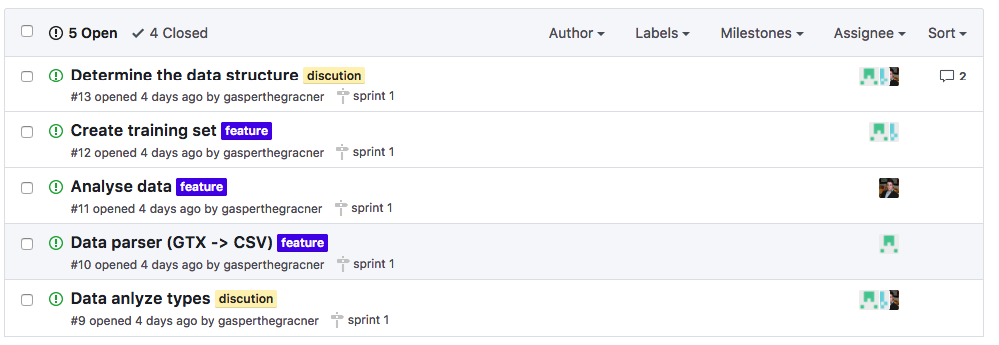
\includegraphics[width=1\textwidth]{issues}
\end{figure}

\end{document}